\documentclass[11pt]{book}
\usepackage[utf8]{inputenc}
\usepackage{tikz}
\usepackage{fancyhdr}
% Estilo de las figuras: es el archivo de sello (`figureCache.stampFiles`).
\tikzset{miestilo/.style={thick,red!60!black}}

% Con guardia: el valor que elige el menú de compilación (el driver lo define antes de cargar esta raíz) tiene que ganar.
\ifdefined\OpcionPie\else\def\OpcionPie{completo}\fi
\pagestyle{fancy}
\fancyhf{}
\fancyfoot[L]{Pie:\OpcionPie}
% La primera página de un capítulo va en estilo `plain`.
\fancypagestyle{plain}{\fancyhf{}\fancyfoot[L]{Pie:\OpcionPie}}

% El libro de estos ejemplos arranca en el capítulo 5: el número impreso no es la posición de la parte.
\setcounter{chapter}{4}

\begin{document}
\chapter{Uno}\label{cap:uno}

Primer capitulo, con una figura.

\begin{figure}[ht]
  \centering
  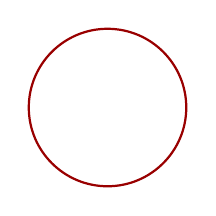
\begin{tikzpicture}
    \draw[miestilo] (0,0) circle (1);
  \end{tikzpicture}
  \caption{Un circulo.}
\end{figure}

\chapter{Dos}\label{cap:dos}

Segundo capitulo: cita al capitulo \ref{cap:uno}.

\chapter{Roto}

Un capitulo con un error a proposito: la exportacion de las demas partes sigue.

\comandoQueNoExiste

\end{document}
